%%%%%%%%%%%%%%%%%%%%%%%%%%%%%%%%%%%%%%%%%
% Beamer Presentation
% LaTeX Template
% Version 1.0 (10/11/12)
%
% This template has been downloaded from:
% http://www.LaTeXTemplates.com
%
% License:
% CC BY-NC-SA 3.0 (http://creativecommons.org/licenses/by-nc-sa/3.0/)
%
%%%%%%%%%%%%%%%%%%%%%%%%%%%%%%%%%%%%%%%%%

%----------------------------------------------------------------------------------------
%	PACKAGES AND THEMES
%----------------------------------------------------------------------------------------


\documentclass{beamer}

\mode<presentation> {
\usetheme{Madrid}

\setbeamertemplate{footline}[page number] % To replace the footer line in all slides with a simple slide count uncomment this line
\setbeamertemplate{navigation symbols}{} % To remove the navigation symbols from the bottom of all slides uncomment this line
}

\usepackage{graphicx} 
\usepackage{booktabs}
\usepackage[T1]{fontenc}
\usepackage{amsmath}
\usepackage{mathtools}
\usepackage{amssymb}
\usepackage{graphicx}
\usepackage{graphics}
\usepackage{algorithmic}
\usepackage{algorithm}
\usepackage{listings}
\graphicspath{ {pictures/} } 

\lstset{ 
	basicstyle=\footnotesize, 
	tabsize=3,
} 
%----------------------------------------------------------------------------------------
%	TITLE PAGE
%----------------------------------------------------------------------------------------

%\title[Short title]{Full Title of the Talk} % The short title appears at the bottom of every slide, the full title is only on the title page
\title[]{Cayley graphs of given degree and diameter on linear groups} % The short title appears at the bottom of every slide, the full title is only on the title page

\author{Mat\'u\v{s} Behun} % Your name
\institute[UCLA] % Your institution as it will appear on the bottom of every slide, may be shorthand to save space
{
Slovak University of Technology in Bratislava \\ % Your institution for the title page
\medskip
%\textit{john@smith.com} % Your email address
}
\date{\today} % Date, can be changed to a custom date

\begin{document}
%------------------------------------------------
\begin{frame}
\titlepage 
\end{frame}
%------------------------------------------------
\begin{frame}
\frametitle{Overview}
\tableofcontents
\end{frame}
%------------------------------------------------
% DEGREE DIAMETER
\section{Degree/diameter problem} 
%------------------------------------------------
\begin{frame}
	\frametitle{Motivation}
\begin{itemize}
    \item In its simplest form, networks can be modeled by graphs with nodes as vertices and links between them as edges.
	\item In modeling interconnection networks by graphs one often considers two restrictions: 
		\begin{itemize}
			\item limitation on the number of physical links leaving a node
			\item limitation on accessibility, that is, any two nodes should be accessible using at most a certain number of physical links. 
		\end{itemize}
		In terms of a graph model this translates into restriction on the maximum degree and on the diameter.
\end{itemize}
\end{frame}
%------------------------------------------------
\begin{frame}
\frametitle{The degree/diameter problem}
	\begin{block}{Degree/diameter problem}
		Find graphs with the largest possible number of vertices, with given degree and diameter.
	\end{block}
	\begin{block}{Edward Forrest Moore}
		Edward Forrest Moore was first who proposed problem of describing and classifying such graphs.
	\end{block}
\end{frame}
%------------------------------------------------
\begin{frame}
	\frametitle{Moore bound}
	There is a theoretical upper bound on the largest order of a graph of maximum degree $d\ge 2$ and diameter $k\ge 1$.
	\begin{equation}\label{eq:Moore}
		\begin{split}
			n_{d,k} \leq M_{d,k}    & = 1 + d + d(d - 1) + \dots + d(d - 1)^{k-1}  \\
									& = 1 + d(1 + (d - 1) + \dots + (d - 1)^{k-1}) \\
									& = \begin{cases}
											1+d\frac{(d-1)^{k}-1}{d-2}, & \text{if}\ d > 2 \\
											2k+1, & \text{if}\ d=2
										\end{cases}
		\end{split}
	\end{equation} ~\\~\\
	Graphs of maximum degree $d$ and diameter $k$ with $M_{d,k}$ vertices are called {\em Moore graphs}. \\~\\
	Moore graphs are necessarily regular.
\end{frame}
%------------------------------------------------
\begin{frame}
	\frametitle{An example of Moore graph}
		\begin{figure}[!ht]
    		\centering
    		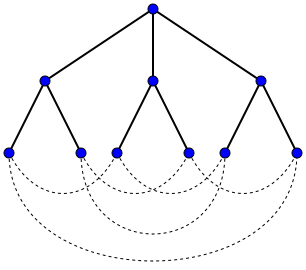
\includegraphics[scale=0.8]{petersen-moore.png}
    		\caption{The Petersen graph is a Moore graph with $d=3$ and $k=2$ }
		\end{figure}
\end{frame}
%------------------------------------------------
\begin{frame}
	\frametitle{Moore graphs}
	Moore graphs are rare; they exist only for the following degrees and diameters: ~\\
	\begin{itemize}
		\item If $d = 2$ for any $k \geq 1$
		\item If $k = 1$ for any $d \geq 2$
		\item If $k = 2$ and $d \in \{3, 7 \}$, and possibly $57$
	\end{itemize} ~\\~\\
	In the remaining cases one tries to construct graphs of maximum degree $d$ and diameter $k$ of order as close to the Moore bound $M_{d,k}$ as possible.
\end{frame}
%------------------------------------------------
\begin{frame}
	\frametitle{Moore graphs}
	\begin{figure}[!ht]
 		\centering
 		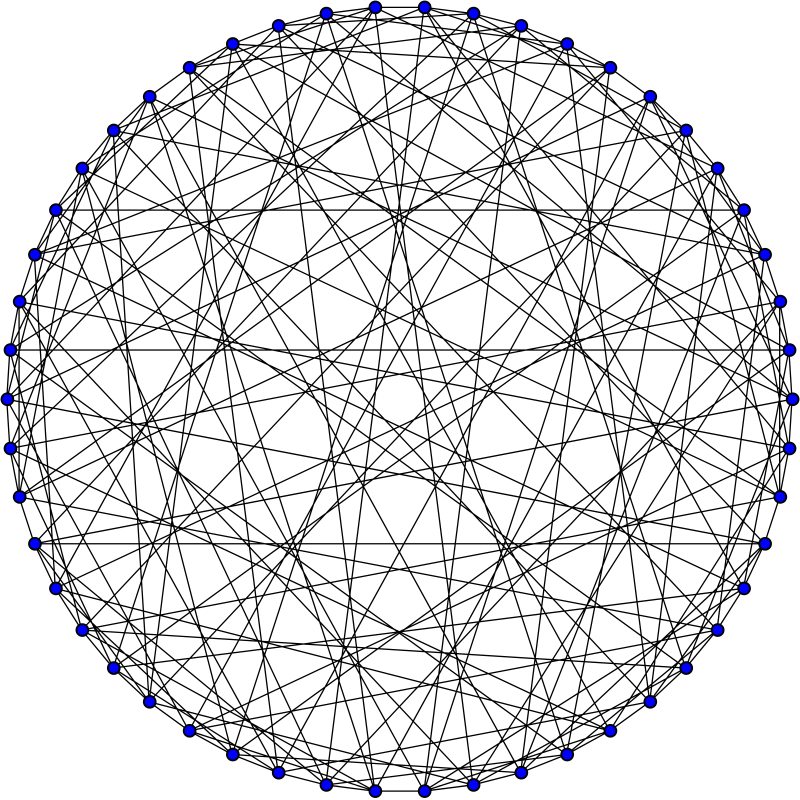
\includegraphics[scale=0.25]{Hoffman-Singleton_graph.png}
		\caption{The Hoffman-singleton graph is Moore graph with $(d,k)=(7,2)$}
	\end{figure}
\end{frame}
%------------------------------------------------
% Graph lifting and Cayley graphs
\section{Cayley graphs} 
%------------------------------------------------
\begin{frame}
	\frametitle{Construction of large $(d,k)$-graphs}
	Finding $(d,k)$-graph of large order is approached by many techniques, mostly using combinatorics on words or various algebraic structures. \\~\\
    We present two examples of bounds arising from such constructions: ~\\
	Using combinatorics on words, Baskoro and Miller(1993) \cite{Bas-Mil} proved that 
    \begin{equation*}
        n_{d,k} \geq \left( \frac{d}{2} \right)^{k} +  \left( \frac{d}{2} \right)^{k-1}     
	\end{equation*}
	With the help of finite fields Bevan, Erskine and Lewis(2017) \cite{Bev-Ers} observed that modified Brown graphs give the bound
    \begin{equation*}
		n_{d,2} \geq d^{2} - 2d^{1+\varepsilon}     
	\end{equation*}
	where $\varepsilon$ depends on results about graphs between consecutive primes.	
\end{frame}
%------------------------------------------------
\begin{frame}
	\frametitle{Cayley graphs}
	Let $\Gamma$ be a group and let $S\subset \Gamma$ be a symmetric unit-free generating set for $\Gamma$; that is, we require that $S=S^{-1}$ and $1\notin S$.\\~\\
	\begin{definition}[Cayley graphs]
		The $\textit{Cayley graph}$ $C(\Gamma,S)$ is the graph with vertex set $\Gamma$ in which vertices $a,b$ are adjacent if $a^{-1}b\in S$.	
	\end{definition} ~\\~\\
	By $C_{d,k}$ we denote the largest order of Cayley graph of degree $d$ and diameter $k$.
	The best currently known lower bound on diameter $2$ for an infinite family of degrees is due to \v{S}iagiov\'a and \v{S}ir\'a\v{n}(2012) \cite{Sia-Sir}: 
	\begin{theorem}
	Let $D = \{ 2^{2m+\mu}+    (2+\delta)2^{m+1}-6,m \geq 1, \mu \in \{0,1\} \}$. Then, for every $d\in D$ one has $C_{d,2} > d^{2} - 6\sqrt{2}d^{3/2}$.
	\end{theorem}
\end{frame}
%------------------------------------------------
\begin{frame}
	\frametitle{General and special linear groups}
		\begin{definition}[General and special linear group] Let $q$ be a power of a prime and let $GF(q)$ be the Galois field of order $q$. The {\em general linear group} $GL(m,q)$ consists of all non-singular $m\times m$ matrices over $GF(q)$ under multiplication. \\~\\
		The special linear group is the subgroup of $GL(m,q)$ consiting of matrices with determinant $1$.
		\end{definition}
		\begin{theorem}[Order of $GL(m,q)$]
			$|GL(m,q)| = (q^m - 1)(q^m - q) \cdots (q^m - q^{m-1})$
		\end{theorem}
		\begin{theorem}[Order of $SL(m,q)$]
			$|SL(m,q)| = |GL(m,q)|/(q-1)$
		\end{theorem}
\end{frame}
%------------------------------------------------
% DEGREE DIAMETER
\section{Computer search} 
%------------------------------------------------
\begin{frame}
	\frametitle{Computer search}
	We created a program generating Cayley graphs of given degree and diameter based on $SL(2,q)$. \\~\\
	As an example, consider the problem of generating a Cayley graph for the group $SL(2,5)$ of diameter $2$ and minimum possible degree: \\~\\

	In order to find graphs with given $d$ and $k$ we generted Cayley graphs from random symmetric unit-free sets $S$ of $SL(2,5)$.
	The order of $SL(2,5)$ is $120$, so that by the Moore bound the first feasible degree (equal to sthe size of a generating set) would be $12$.
\end{frame}
%------------------------------------------------
\begin{frame}
	\frametitle{Computer search}
	 The group $SL(2,5)$ has only one involution; all the remaining $118$ elements form $59$ pairs of the form $\{x,x^{-1}\}$. \\~\\
	 To check all Cayley graphs $C(G,S)$ for $G=SL(2,5)$ and $|S|=12$ we would have to generate all the ${59 \choose 6} = 45057474$ possibilities for $S$ and then check for the diameter of the resulting Cayley graphs. \\~\\
	For the group $G=SL(2,5)$ and generating sets $S$ such that $|S|=d$ by our randomized algorithm we found the following number of generating sets giving Cayley graphs $C(G,S)$ of diameter $2$: \\~\\
	\begin{tabular}[htbp]{l*{10}{c}r}
		$d$ & $13$ & $14$ & $15$ & $16$ & $17$ & $18$ & $19$ & $20$ & $21$ \\
		\hline
 		Found graphs & $0$  & $0$ & $1$ & $107$ & $345$ & $2451$  & $4120$ & $11669$ & $14926$ \\
	\end{tabular} 
\end{frame}
%------------------------------------------------
\begin{frame}
	\frametitle{Algorithm for generation of cayley graph}
	\lstinputlisting[language=Perl]{while.pl}
\end{frame}
%------------------------------------------------
\begin{frame}
	\frametitle{Algorithm for diameter}
	\lstinputlisting[language=Perl]{diameter.pl}
\end{frame}
%------------------------------------------------
\begin{frame}
	\frametitle{An example of the output for $SL(2,3)$}
	\begin{figure}[!ht]
 		\centering
 		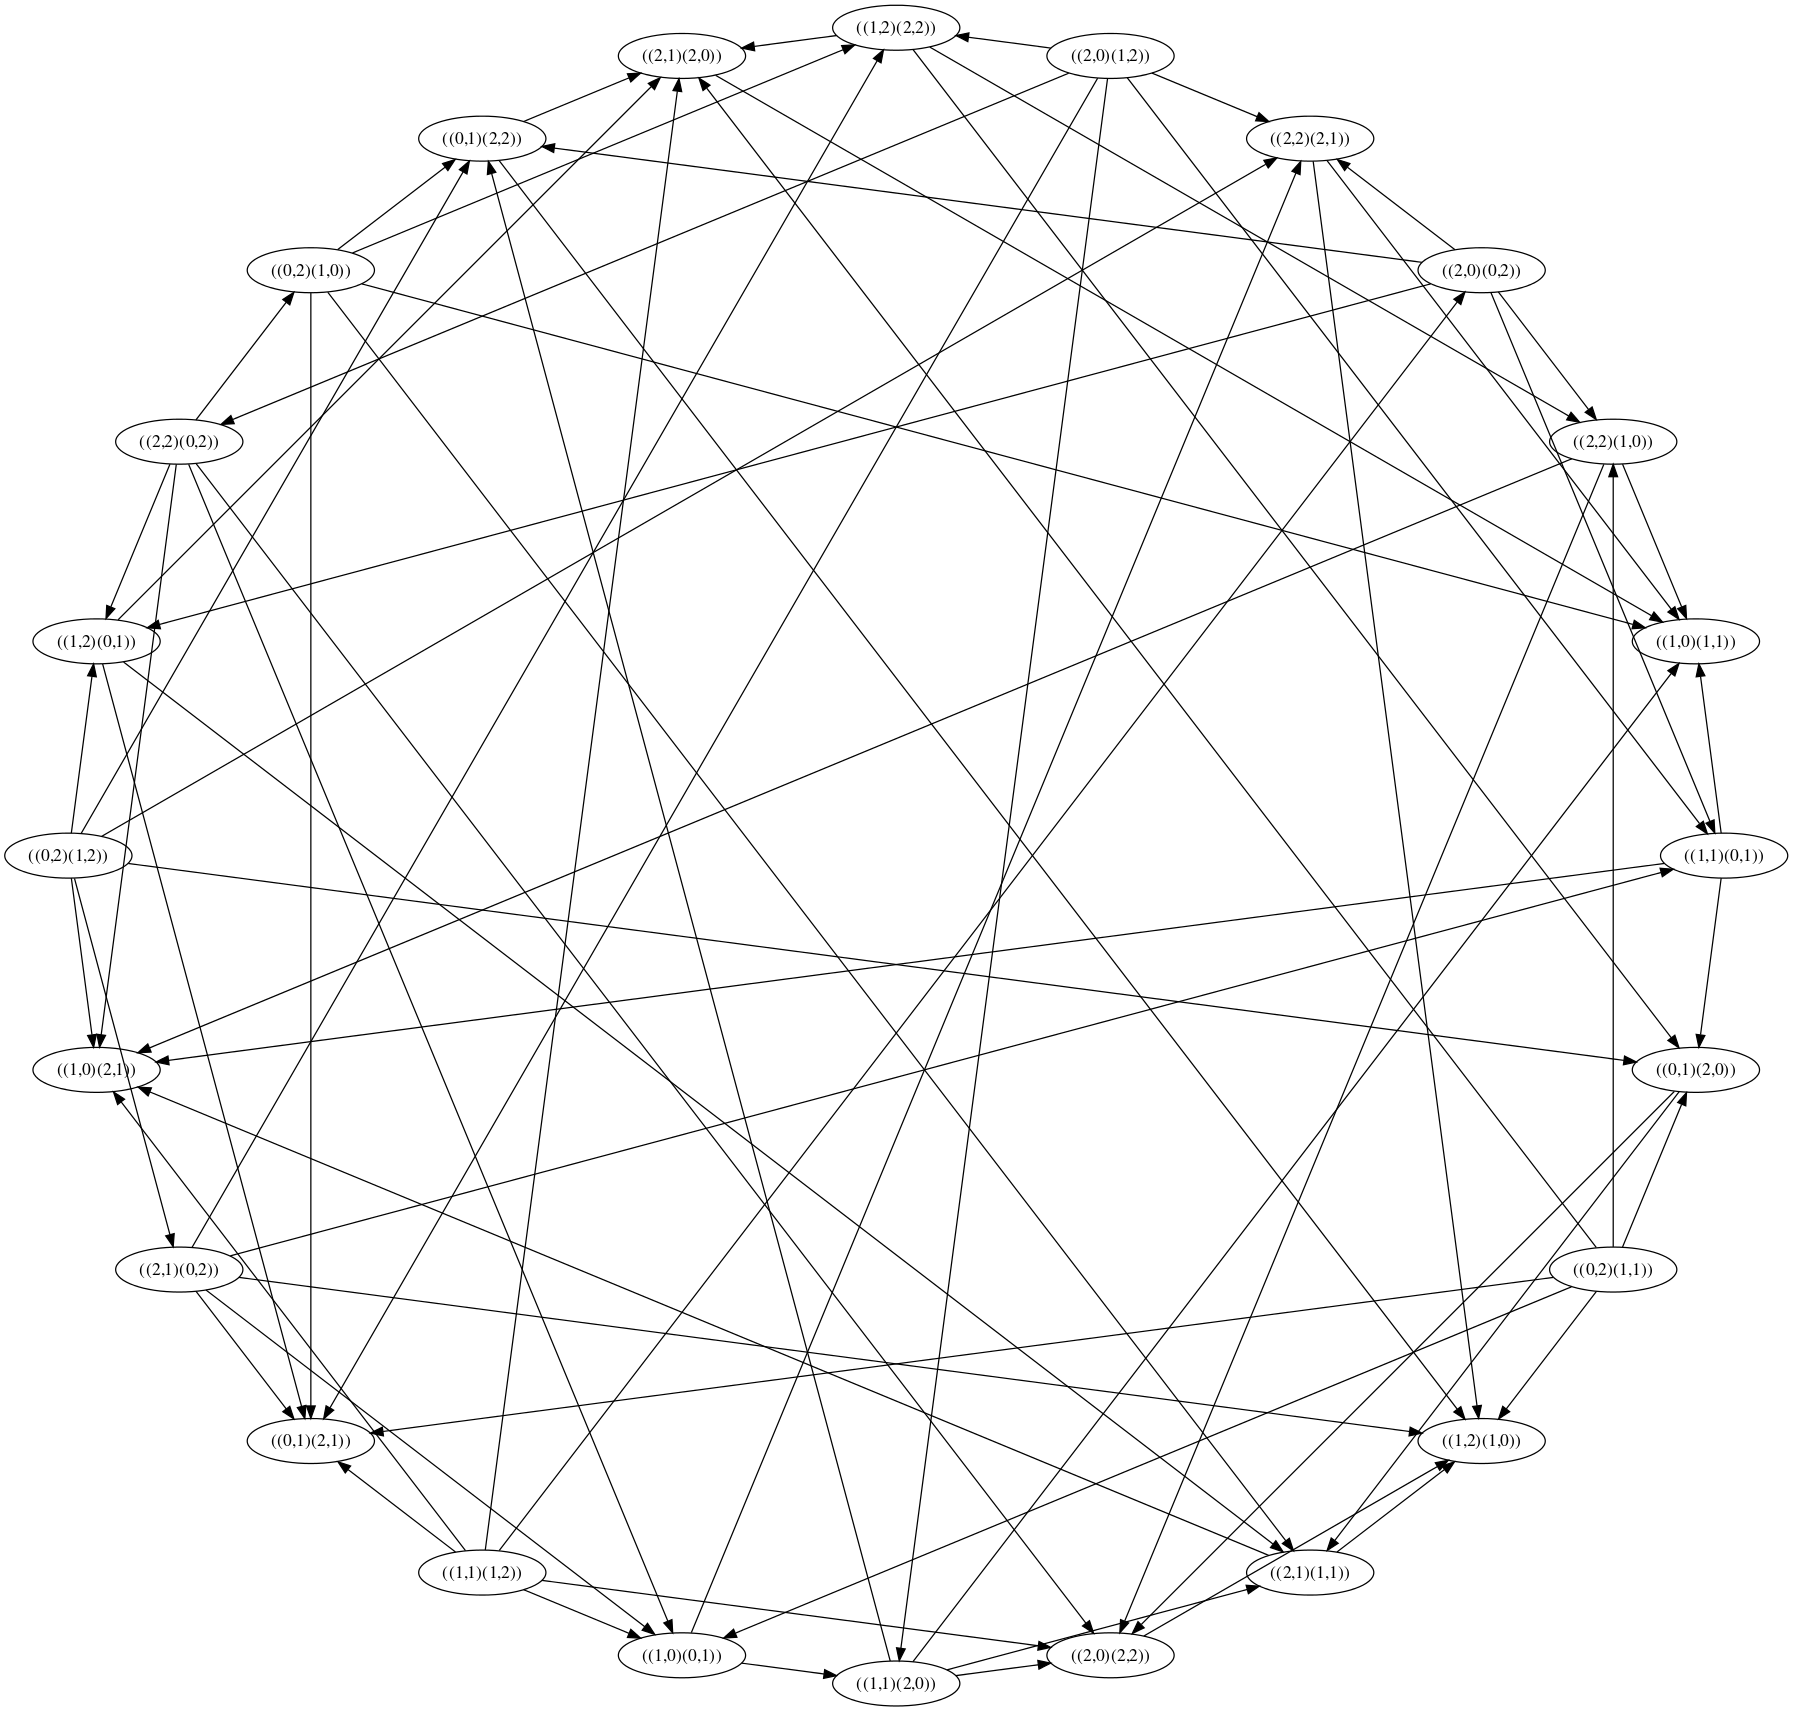
\includegraphics[scale=0.12]{example.png}
		\caption{One of the generated graphs from $SL(2,3)$ }
	\end{figure}
\end{frame}
%------------------------------------------------
\begin{frame}
	\frametitle{Further research}
	\begin{itemize}
		\item Finding regular graphs of a given degree and girth of the smallest possible order is known as the degree/girth problem. With small changes to program we can systematically or randomly look for Cayley graphs and check its girth.
		\item Applying our algorithm to generate graphs of diameter $2$ and comparably small degree that are Cayley graphs of $SL(2,q)$ for $q>5$.
	\end{itemize}
\end{frame}
%------------------------------------------------
\begin{frame}
	\frametitle{References}
    \footnotesize{
    	\begin{thebibliography}{99} % Beamer does not support BibTeX so references must be inserted manually as below
			\bibitem{Bas-Mil} E. T. Baskoro and M. Miller, On the construction of networks with minimum diameter,
				Australian Computer Science Communications C 15 (1993) 739?743.

			\bibitem{Bev-Ers} D. Bevan, G. Erskine and R. Lewis, Large circulant graphs of fized diameter and arbitrary degree, Ars Math. ontemp. 13 (2017), 275--29.
			\bibitem{Sia-Sir} J. \v{S}iagiov\'a and J. \v{S}ir\'a\v{n}, Approaching the Moore bound for diameter two by Cayley graphs, J. Combin. Theory Ser. B 102 (2012) 470--4    73.
        \end{thebibliography}
    }
\end{frame}
%------------------------------------------------
\begin{frame}
\Huge{\centerline{The End}}
\end{frame}
%----------------------------------------------------------------------------------------
\end{document} 
\begin{frame}
	\frametitle{Computer search of Cayley graphs}
	We know that Cayley graph is lift of one vertex with $|S|$ edges. We exploit that property by computation of diameter on smaller graph to determine it.
	\begin{theorem}[Diameter of Cayley graph]
		Cayley graph $(\Gamma, S)$ has diameter $k$ if and only if \\
		$ \forall x \in Cay(\Gamma, S) there \exists x_{1}, x_{2}, \dots ,x_{i} \in S$
	\end{theorem}
\end{frame}
%------------------------------------------------
\begin{frame}
	\frametitle{Graph lifting}
	Let $G$ be an undirected graph. We will assign direction to every edge of graph and making them {\em arcs}. {\em Arc} with {\em reversed} direction of $e$ is denoted by $e^{-1}$. 
	\begin{definition}[Graph lifting]
		Let $G$ be a graph as above and let $\Gamma$ be a finite group. The mapping
		\begin{align*}
			\alpha: D(G) \rightarrow \Gamma
		\end{align*}
		will be called a {\em voltage assignment} if $\alpha(e^{-1})$ = $(\alpha(e))^{-1}$, for any arc $e \in D(G)$.
	\end{definition}
\end{frame}
%------------------------------------------------
\begin{frame}
	\frametitle{Graph lifting example}
		\begin{itemize}
			\item A {\em walk} of length $\ell$ in $G$ is any sequence $W=e_1e_2\ldots e_{\ell}$ of consecutive arcs of $G$, and the voltage $\alpha(W)$ of the walk is simply the product $\alpha(W)=\alpha(e_1)\alpha(e_2)\cdots \alpha(e_{\ell})$. \\
			\item Lift $G^{\alpha}$ has diameter at most $k$ if for any two vertices $u,v$ of $G$ and for any element $g\in \Gamma$ there is a walk $W$ of length at most $k$ emanating from $u$ and terminating at $v$ such that $\alpha(W)=g$; in the case when $u=v$ we also require that $g\ne 1$.
		\end{itemize}
 		Obrazok zdvihu na petersenov graf.

\end{frame}
